\documentclass[french, 11pt]{article}

\input{/home/theo/MP2I/setup.tex}

\usetikzlibrary{automata, positioning}

\renewcommand*{\S}{\Sigma}
\newcommand*{\Reg}{\nt{Reg}}
\renewcommand*{\V}{\mathcal{V}}
\renewcommand*{\R}{\mathcal{R}}
\renewcommand*{\ra}{\Rightarrow}

\def\chapitre{2}
\def\pagetitle{Langages et Mots.}

\begin{document}

\input{/home/theo/MP2I/title.tex}

\begin{defi}{}{}
    On considère un alphabet $\S$ et on appelle mot une suite d'éléments de $\S$.\\
    Un élément de $\S$ est appelé une lettre. 
\end{defi}

\begin{defi}{}{}
    On appelle langage sur $\S$ un ensemble de mots sur l'alphabet $\S$.
\end{defi}

\section{Expressions régulières.}

\begin{defi}{}{}
    Les expressions régulières sur $\S$ sont définies inductivement.\\
    --- $\forall a \in \S$, $a$ est une expression régulière.\\
    --- $\e$ et $\0$ sont des expressions régulières.\\ 
    --- $e_1\mid e_2$ est une expression régulière si $e_1$ et $e_2$ en sont.\\
    --- $e_1e_2$ est une expression régulière si $e_1$ et $e_2$ en sont.\\
    --- $e_1^*$ aussi.
\end{defi}

\begin{defi}{}{}
    À chaque expression régulière $e$, on souhaite associer un langage $L(e)$.\\
    Il est défini inductivement :\\
    --- $L(a)=\{a\}$.\\
    --- $L(\0)=\0$.\\
    --- $L(\e)=\{\e\}$ le mot vide.\\
    --- $L(e_1e_2)=L(e_1)L(e_2)$.\\
    --- $L(e_1\mid e_2)=L(e_1)\cup L(e_2)$.\\
    --- $L(e_1^*)=\bigcup_{i=0}^{+\infty}L(e_1)^i$, appelé étoile de Kleene.
\end{defi}

\begin{defi}{}{}
    Deux expressions régulières $e_1$ et $e_2$ sont équivalentes si $L(e_1)=L(e_2)$. 
\end{defi}

\begin{ex}{}{}
    Si $e$ est une expression régulière, alors :\\
    --- $e\mid\0\sim e$.\\
    --- $e\0\sim\0$.\\
    --- $\0^*=\e$.
\end{ex}

\begin{prop}{}{}
    Si $e$ est une expression régulière, il existe $e'$ qui n'utilise pas $\0$ telle que $e\sim e'$ ou $e\sim\0$.
    \tcblower
    -- Si $e=a$, avec $a\in\S$, alors $e'=a$ convient.\\
    -- Si $e=\e$, alors $e'=\e$ convient.\\
    -- Si $e=\0$, alors n'importe quel $e'$ convient.\\
    -- Si $e=e_1\mid e_2$, par induction, $e_1\sim e_1'$ ou $e_1\sim\0$, de même pour $e_2$.\\
    --- Si $e_1\sim e_1'$ et $e_2 \sim e_2'$, alors $e\sim e_1'\mid e_2'$ n'utilise pas $\0$.\\
    --- Si $e_1\sim e_1'$ et $e_2\sim\0$, alors $e\sim e_1'$.\\
    --- Si $e_1\sim \0$ et $e_2\sim \0$, alors $e\sim\0$.\\
    -- Si $e=e_1\cdot e_2$, alors $e\sim \0$ ssi $e_1\sim \0$ ou $e_2\sim \0$.\\
    -- Si $e=e_1^*$, alors $e=\e$ si $e_1\sim\0$, sinon $e=e_1'^*$ si $e_1\sim e_1'$.
\end{prop}

\begin{corr}{}{}
    À part pour décrire le langage vide, le symbole $\0$ est inutile dans la définition des expression régulières.
\end{corr}

\begin{prop}{}{}
    Si $e$ est une expression régulière sans $\0$, alors il existe $e'$ sans $\e$ tel que :\\
    --- $e'\sim e$ ou $e\sim e'\mid\e$ ou $e\sim \e$.
\end{prop}

\begin{ex}{}{}
    Trouver des expressions régulières pour :\\
    --- L'ensemble des mots de $\{a,b\}$ qui contiennent un nombre pair de $a$.\\
    --- L'ensemble des mots de $\{a,b\}$ qui ne contient pas deux $a$ d'affilée.\\
    --- L'ensemble des mots de taille 3.
    \tcblower
    \boxed{1.} $(ab^*a\mid b^*)^*$\\
    \boxed{2.} $a\mid(b \mid ab)^*(a\mid \e)$.\\
    \boxed{3.} $(a\mid b)(a\mid b)(a\mid b)$.
\end{ex}

\begin{prop}{}{}
    On a $|\Sigma|^k$ mots de taille $k$.
\end{prop}

\begin{prop}{}{}
    Si $L$ est un langage fini de taille finie, il existe une expression régulière $e$ telle que $L(e)=L$.
\end{prop}

\begin{defi}{}{}
    On dit d'un langage qu'il est régulier s'il existe une expression qui le caractérise.
\end{defi}

\begin{prop}{}{}
    Il existe des langages non réguliers.
    \tcblower
    Un langage peut être vu comme un élément de $\{0,1\}^\N$. La valeur $i$ indique si le $i$ème mot appartient au langage.
\end{prop}

\begin{defi}{}{}
    On définit $\Reg(\S)$ comme l'ensemble des langages réguliers sur $\S$.
\end{defi}

\begin{prop}{}{}
    On a $\Reg(\S)$ le plus petit ensemble de langages contenant $\{\e\},\0,\{a\}$ qui soit stable par union, concaténation et étoile de Kleene.
    \tcblower
    Montrons que $\Reg(\S)$ vérifie ces propriétés.\\
    --- $\{\e\}\in\Reg(\S)$ car caractérisé par $\e$, de même pour $\{a\}$ et $\0$.\\
    --- Soient $L_1,L_2\in\Reg(\S)$. Il existe $e_1,e_2$ deux expressions régulières telles que $L(e_1)=L_1$ et $L(e_2)=e_2$.\\
    Alors $L(e_1\mid e_2)=L(e_1)\cup L(e_2)=L_1\cup L_2$; $L(e_1e_2)=L_1L_2$ et $L(e_1^*)=L_1^*$.\\
    --- Soit $X$ un ensemble de langages vérifiant ces propriétés. On va réaliser une induction sur les langages réguliers.\\
    Soit $L\in\Reg(\S)$ et $e$ une expression régulière qui le caractérise.\\
    --- Si $e\in\{\0,\e,a\}$, alors $L\in X$.\\
    --- Si $e=e_1\mid e_2$, alors $L_1,L_2\in X$, puis $L(e)=L(e_1)\cup L(e_2)\in X$.\\
    --- Si $e=e_1e_2$, alors $L_1,L_2\in X$, puis $L(e)=L(e_1)L(e_2)\in X$.\\
    --- Si $e=e_1^*$, alors $L_1\in X$, puis $L(e)=\bigcup_k L(e_i)^k$.\\
    Donc $\Reg(\S)\in X$.
\end{prop}

\section{Automates finis.}

\begin{defi}{}{}
    Un automate est un quintuplet $(\S,Q,q_0,F,\d)$ où :\\
    --- $\S$ est l'alphabet.\\
    --- $Q$ est l'ensemble des états.\\
    --- $q_0\in Q$ est l'état initial.\\
    --- $F\subset Q$ est l'ensemble des états finaux.\\
    --- $\d:Q\times\S\to Q$ est la fonction de transition.
\end{defi}

\begin{ex}{}{}
    \begin{center}
        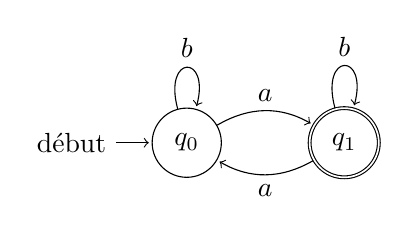
\begin{tikzpicture}[shorten >=1pt, node distance=2cm, on grid, auto, initial text = \nt{début}] 
            \node[state,initial] (q_0)   {$q_0$}; 
            \node[state, accepting] (q_1) [right=of q_0] {$q_1$}; 
            \path[->] 
            (q_0) edge [bend left] node {$a$} (q_1)
                edge [loop above] node {$b$} ()
            (q_1) edge [loop above] node {$b$} ()
                edge [bend left] node {$a$} (q_0);
        \end{tikzpicture}
    \end{center}
    Si un mot est accepté, il contenait un nombre impair de $a$, sinon il en contenait un nombre pair.\\
    Alors : $\S=\{a,b\}$, $Q=\{q_0,q_1\}$, $F=\{q_1\}$ et :
    \begin{eqnarray*}
        \begin{array}{|c|c|c|}
            \hline
            Q\setminus \S& a & b\\
            \hline
            q_0 & q_1 & q_0\\
            \hline
            q_1 & q_0 & q_1\\
            \hline
        \end{array}
    \end{eqnarray*}
\end{ex}

\begin{defi}{}{}
    On étend la défintiion de $\d$ de la façon suivante :
    \begin{enumerate}
        \item $\forall q \in Q, ~ \d^*(q,\e)=q$.
        \item $\forall q \in Q, ~ \forall a \in \S, ~ \forall m \in \S^*, ~ \d^*(q,am)=\d^*(\d(q,a),m)$.
    \end{enumerate}
    Un mot $m$ est dit accepté par l'automate $A=(\S,Q,q_0,F,\d)$ si $\d^*(q_0,m)\in F$.
\end{defi}

\begin{defi}{}{}
    Si $A$ est un automate, on note $L(A)$ l'ensemble des mots acceptés par $A$, le langage reconnu par $A$.
\end{defi}

\begin{ex}{}{}
    Montrons que $L_A=\{m\in\S^*, ~ |m|_a \equiv 1[2]\}$, où $|m|_a$ est le nombre de $a$ dans $m$.
    \tcblower
    Par récurrence, $\P_n$ : << $\forall q_i \in Q, ~ \forall m \in \S^*, ~ \d^*(q_i,m)=q_j$ où $j\equiv i+|m|_a[2]$ >>.\\
    \bf{Initialisation.} On a $\d^*(q_i,\e)=q_i$ et $i\equiv i+0[2]$.\\
    \bf{Hérédité.} Soit $n\in\N$ tel que $\P_n$. Soit $m=cm'$ de taille $n+1$, alors $\d^*(q_i,m)=\d^*(\d(q_i,c),m')$.\\
    -- Si $c=a$, alors $\d(q_i,c)=q_j$ avec $j\equiv i+1[2]$, donc $\d^*(q_j,m')=q_{j'}$ où $j'\equiv j+|m'|_a[2]=i+|m|_a[2]$.\\
    -- Si $c=b$, alors $\d(q_i,c)=q_i$ donc $\d^*(q_i,m)=\d^*(q_i,m')=q_j$ avec $j\equiv i+|m'|_a[2]=i+|m|_a[2]$.\n
    On traite le cas $q_i=q_0$ : $\forall m \in \S^*, ~ \d^*(q_0,n)=q_j$ avec $j=|m|_a[2]$.\\
    Le mot est accepté ssi $j=1$ ssi $|m|_a\equiv1[2]$ donc $L_A=\{m\in\S^*,~|m|_a\equiv1[2]\}$.\n
    On pourrait définir $\tilde{\d^*}(q,\e)=q$ et $\tilde{\d^*}(q,ma)=\d(\tilde{\d^*}(q,m),a)$.
\end{ex}

\begin{defi}{}{}
    On dit d'un état $q$ qu'il est accessible s'il existe un mot $m$ tel que $\d^*(q_0,m)=q$.
\end{defi}

\begin{defi}{}{}
    Un état est dit co-accessible s'il existe un mot $m$ tel que $\d^*(q,m)\in F$.
\end{defi}

\begin{defi}{}{}
    Un état est utile s'il est accessible et co-accessible.\\
    Un automate est dit émondé si tous ses états sont utiles.\\
    La fonction de transition n'est définie que partiellement.\\
    Le langage des mots acceptés est celui des mots $m$ tels que $\d^*(q_0,m)$ est défini et dans $F$.\\
    Si la fonction de transition est définie sur tout $Q\times\S$, on dit que l'automate est complet.
\end{defi}

\begin{defi}{}{}
    Pour compléter un automate, on peut ajouter un état $q_p$ et on complète la fonction de transition :
    \begin{equation*}
        \forall q \in Q, ~ \forall a \in \S, \nt{si } \d(q,a) \nt{ n'est pas défini, } \d(q,a):=q_p.
    \end{equation*}
    \begin{equation*}
        \forall a \in \S, ~ \d(q_p,a):=q_p.
    \end{equation*}
\end{defi}

\begin{defi}{Automate non déterministe.}{}
    Un automate non déterministe est un quintuplet : $(\S,Q,I,F,\d)$, et $\d:Q\times\S\to\P(Q)$.\\
    Un mot est accepté par l'automate s'il existe un chemin d'un état initial à un état final qui soit étiqueté par $m$.\\
    On cherche à étendre $\d$ aux mots de $\S^*$ :\\
    --- $\forall q \in Q, ~ \d^*(q,\e)=\{q\}$.\\
    --- $\forall q \in Q, ~ \forall a \in \S, \forall m \in \S^*, \d^*(q,am)=\bigcup_{q_i\in\d(q,a)}\d^*(q_i,m)$.
\end{defi}

\begin{prop}{}{}
    On peut transformer un automate déterministe en non-déterministe.\\
    Il suffit de prendre $I=\{q_0\}$ et $\d'(q,a)=\{\d(q,a)\}$.\n
    L'opération inverse est possible.
\end{prop}

\vspace*{0.3cm}

\begin{defi}{}{}
    Soit $A=(\S,Q,I,F,\d)$ non déterministe, on définit $A'$ de la façon suivante :\\
    --- $\S$ est le même.\\
    --- $Q'=\P(Q)$.\\
    --- $q_0=I$.\\
    --- $F'=\{E\in\P(Q), ~ E\cap F \neq \0\}$.\\
    --- $\d'(E,a)=\bigcup_{q\in E}\d(q,a)$. (l'union des états atteignables par une lettre $a$ depuis un état de $E$).\\
    On appelle ce procédé la déterminisation d'un automate.\\
    En pratique, on ne fait apparaître que les éléments de $\P(Q)$ par lesquels on passe.\\
    L'automate produit par ce procédé a un nombre d'états exponentiel en celui de l'automate initial.
\end{defi}

\vspace*{0.3cm}

\begin{ex}{}{}
    On considère $L_n$ le langage des mots de $\{a,b\}^*$ qui contiennent un $a$ $n$ lettres avant la fin.\\
    Construire un automate non-déterministe, puis déterministe qui reconnaît les mots de $L_3$.
    \tcblower
    \phantom{a}
    \begin{center}
        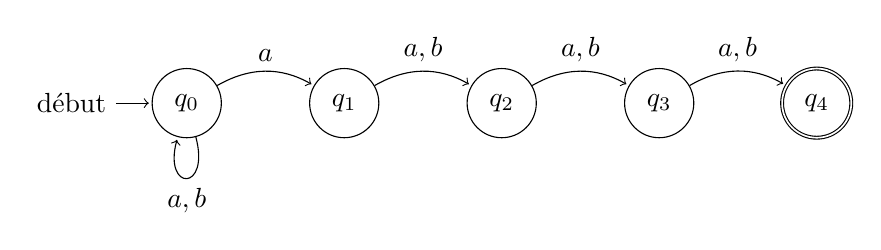
\begin{tikzpicture}[shorten >=1pt, node distance=2cm, on grid, auto, initial text = \nt{début}] 
            \node[state,initial] (q_0)   {$q_0$}; 
            \node[state] (q_1) [right=of q_0] {$q_1$}; 
            \node[state] (q_2) [right=of q_1] {$q_2$}; 
            \node[state] (q_3) [right=of q_2] {$q_3$}; 
            \node[state, accepting] (q_4) [right=of q_3] {$q_4$}; 
            \path[->] 
            (q_0) edge [loop below] node {$a,b$} ()
                edge [bend left] node {$a$} (q_1)
            (q_1) edge [bend left] node {$a,b$} (q_2)
            (q_2) edge [bend left] node {$a,b$} (q_3)
            (q_3) edge [bend left] node {$a,b$} (q_4);
        \end{tikzpicture}
    \end{center}
\end{ex}

\vspace*{0.3cm}

\begin{prop}{}{}
    Tout automate déterministe reconnaissant $L_n$ a au moins $2^{n+1}$ états.
    \tcblower
    On considère $u$ et $v$ deux mots de $\S^{n+1}$. Montrons que $u\neq v \ra \d^*(q_0,u)\neq d^*(q_0,v)$.\\
    Supposons $u\neq v$, alors $\exists (u_1,u_2),(v_1,v_2), ~ u=u_1au_2$ et $v=v_1bv_2$, avec $|u_1|=|v_1|$ et $|u_2|=|v_2|$.\\
    Soit $w$ le mot $a^{n-|u_2|}$, alors $uw=u_1au_2w$ et $|u_2|+|w|=n$ donc $uw$ est accepté, et $vw$ ne l'est pas.\\
    Alors $\d^*(q_0,uw)\in F$ et $\d^*(q_0,vw)\notin F$, or $\d^*(q_0,uw)=\d^*(\d^*(q_0,u),w)$ et $\d^*(q_0,vw)=\d^*(\d^*(q_0,v),w)$.\\
    On a donc $\d^*(q_0,u)\neq\d^*(q_0,v)$, donc $\d^*$ est injective de $\S^{n+1}$ vers $Q$ donc $|Q|\geq|\S^{n+1}|=2^{n+1}$.
\end{prop}

\vspace*{0.3cm}

\begin{defi}{}{}
    Le passage au miroir de $L$, noté $\ov{L}$ est l'ensemble $\{\ov{w}, ~ w \in L\}$, où $\ov{w}$ est $w$ lu à l'envers.
\end{defi}

\vspace*{0.3cm}

\begin{prop}{}{}
    L'ensemble des langages reconnus par des automates est stable par intersection.
    \tcblower
    Soient $A_1=(\S_1,Q_1,q_0^1,F_1,\d_1)$, $A_2=(\S_2,Q_2,q_0^2,F_2,\d_2)$ deux automates déterministes sans perte de généralité.\\
    Soient $L_1$ et $L_2$ les langages reconnus par $A_1$ et $A_2$. On cherche un automate reconnaissant $L_1\cap L_2$.\\
    Soit $w\in L_1\cap L_2$ : $\d^*(q_0^1,w)\in F_1$ et $\d^*(q_0^2,w)\in F_2$. On pose :
    \begin{equation*}
        \S = \S_1 \cup \S_2, ~ Q = Q_1 \times Q_2, ~ q_0 = (q_0^1, q_0^2), ~ F=F_1\times F_2, ~ \et ~ \d: \begin{cases} Q_1 \times Q_2 \times \S &\to \quad Q_1 \times Q_2 \\ (q_1,q_2,a) &\mapsto \quad  (\d_1(q_1,a),\d_2(q_2,a)) \end{cases}
    \end{equation*}
    Par récurrence sur la taille de $w$, $\d^*((q_0^1, q_0^2), w) = (\d_1^*(q_0^1,w), \d_2^*(q_0^2,w))$.\\
    On définit $A=(\S, Q, q_0, F, \d)$. On a alors :
    \begin{align*}
        w \in L(A) &\iff \d^*((q_0^1,q_0^2),w) \in F_1\times F_2 \\
        &\iff (\d_1^*(q_0^1,w),\d_2^*(q_0^2,w))\in F_1\times F_2\\
        &\iff \d_1^*(q_0^1,w) \in F_1 ~\et~ \d_2^*(q_0^2,w) \in F_2\\
        &\iff w\in L_1 \cap L_2.
    \end{align*}
    Donc $L(A)=L_1\cap L_2$.
\end{prop}

\pagebreak

\begin{prop}{}{}
    L'ensemble des langages reconnus par des automates est stable par passage au miroir.
    \tcblower
    Soit $A=(\S,Q,q_0,F,\d)$ un automate déterministe et complet qui reconnaît $L$.\\
    On définit $A'=(\S,Q,F,q_0,\d')$, avec $\forall (q,a) \in Q\times \S, ~ \d(q,a)=q' \ra q \in \d'(q',a)$ (on retourne les flèches).\\
    Par récurrence sur la taille de $w$, $\forall q \in Q, ~ \forall w \in \S^*, ~ \d^*(q,w)=q' \iff q \in \d'^*(q',\ov{w})$.
    \begin{align*}
        w \in L &\iff \exists q_F \in F, ~ \d^*(q_0,w) = q_F  \iff q_0 \in \d'^*(q_F, \ov{w})\\
        &\iff q_0 \in \bigcup_{q_F \in F} d^*(q_F, \ov{w}) \iff \ov{w}\in L(A').
    \end{align*}
    Donc $L(A')=\ov{L}$.
\end{prop}

\vspace*{0.3cm}

\begin{defi}{Algorithme d'élimination des états.}{}
    \boxed{1.} Ajouter $\a$ et $\w$ deux nouveaux états, $\a$ nouvel initial, $\w$ nouvau final.\\
    L'automate ainsi produit a des transitions étiquetées avec des expressions régulières.\\
    \boxed{2.} Éliminer un état, différent de $\a$ et $\w$, et reporter ses transitions.\\
    \boxed{3.} Répéter jusqu'à ce qu'il ne reste que $\a$ et $\w$.\\
    L'expression régulière finale, reliant $\a$ et $\w$ caractérise le langage reconnu par l'automate.
    \tcblower
    L'algorithme termine car $|Q|$ est un variant. Il est correct car les langages reconnus par les automates intermédiaires sont les mêmes.
\end{defi}

\vspace*{0.3cm}

\begin{defi}{}{}
    Un automate est dit généralisé si ses transitions sont étiquetées par des expressions régulières.
\end{defi}

\vspace*{0.3cm}

\begin{defi}{}{}
    Un mot $m$ est accepté par un automate généralisé s'il existe un chemin d'un état initial vers un état final étiqueté par une expression régulière $e$ telle que $m\in L(e)$.
\end{defi}

\vspace*{0.3cm}

\begin{defi}{}{}
    Soit $L$ un langage, on définit :\\
    --- $P(L) = \{e \in \S, ~ \exists n \in \S^*, ~ en \in L\}$, l'ensemble des préfixes de $L$.\\
    --- $D(L) = \{e \in \S, ~ \exists n \in \S^*, ~ ne \in L\}$, l'ensemble des suffixes de $L$.\\
    --- $F(L) = \{u \in \S^2, ~ \exists n_1,n_2 \in \S^*, ~ n_1un_2\in L\}$, l'ensemble des facteurs de $L$ de taille 2.
\end{defi}

\vspace*{0.3cm}

\begin{defi}{}{}
    Un langage est dit local si $L\setminus\{\e\}=(P(L)\S^*\cap\S^*D(L)) \setminus (\S^*(\S^2\setminus F(L))\S^*)$.\\
    Ce sont les mots qui commencent et finissent comme un mot de $L$, et qui ne possèdent pas de facteur de taille 2 qui n'est pas un facteur de $L$.
\end{defi}

\vspace*{0.3cm}

\begin{prop}{}{39}
    Si un langage est local, il est reconnaissable par un automate.
    \tcblower
    Soit $Q=\S\cup\{\e\}$, $q_0=\e$ et $F=D(L)$, $\forall e \in P(L), ~ \d(q_0,e)=e$, $\forall e_1e_2\in F(L), ~ \d(e_1,e_2)=e_2$.\\
    $q$ représente la dernière lettre lue. Si on a aucune lettre, on est en $\e$, et pour accepter un mot, la prochaine lettre lue doit appartenir à $D(L)$.\\
    Si on est en $e_1$, la prochaine lettre lue doit former un élément de $F(L)$ lorsqu'elle est concaténée à $e_1$.\\
    Cet automate reconnaît le langage $(P(L)\S^*\cap\S^*D(L))\setminus(\S^*(\S^2\setminus F(L))\S^*)$.\\
    Si $L$ est local, on peut construire cet automate pour reconnaître $L\setminus\{e\}$.\\
    Si $\e\in L$, on rajoute simplement $\e$ aux états finaux.
\end{prop}

\vspace*{0.3cm}

\begin{defi}{}{}
    Une expression régulière est dite linéaire si chaque lettre de $\S$ apparaît au plus une fois.
\end{defi}

\begin{prop}{}{}
    Si $e$ est une expression régulière linéaire, alors $L(e)$ est un langage local.
    \tcblower
    Par induction :\\
    --- $\0$ ou $\e$ : $P(L)=F(L)=D(L)=\0$.\\
    --- $a$ : $P(L)=D(L)=\{a\}$ et $F(L)=\0$.\\
    --- $e_1e_2$ : $P(L)=P(L_1)\cup P(L_2)$ si $\e\in L_1$, sinon $P(L_1)$, pareil pour $D(L)$.\\
    Traitons le cas où $\e \notin P(L_1)$, et $\e\notin D(L_2)$. On a $m$ commence par une lettre de $P(L_1)$ et termine par $D(L_2)$.\\
    Alors $m=m_1...m_n$, et $\exists i$ tel que $m_i$ est une lettre utilisée pour $e_1$, et $m_{i+1}$ est utilisée pour $e_2$.\\
    Alors $n_i \in D(L_i)$ et $n_{i+1}\in P(L_2)$, et $\forall k < i, ~ m_km_{k+1}\in F(L_1)$, et $\forall k \in \lb i+1,n-1\rb$, $m_km_{k+1} \in F(L_2)$.\\
    On a $m_im_{i+1}\in D(L_1)P(L_2)$ puis $m_1...m_i \in L_1 \setminus{\e}$ par induction, $L_1$ étant local.\\
    Alors $m_{i+1}...m_n \in L_2\setminus\{\e\}$ par induction et $m\in L_1L_2=L(e)$. 
\end{prop}

\begin{defi}{Algorithme de Berry-Sethi.}{}
    \begin{algorithm}[H]
        \caption{Algorithme de Berry-Sethi.}
        \Entree{Une expression régulière $e$.}
        1 - Linéariser $e$ en $e'$.\\
        2 - Calculer $D(L)$, $P(L)$ et $F(L)$.\\
        3 - Construire l'automate (\ref{prop:39}).\\
        4 - Délinéariser.\\
        5 - Déterminiser.
    \end{algorithm}
\end{defi}

\begin{corr}{}{}
    Tout langage caractérisé par une expression régulière est reconnaissable par un automate.
\end{corr}

\begin{corr}{}{}
    Les langages réguliers sont stables par intersection et passage au miroir.
\end{corr}

\begin{exercice}{}{}
    Les langages réguliers sont stables par complémentaire.
\end{exercice}

\begin{thm}{de Kleene.}{}
    Les langages reconnus par des automates sont exactement les langages réguliers.
    \tcblower
    \boxed{\ra} Prouvé par l'algorithme d'élimination des états.\\
    \boxed{\la} Prouvé par l'algorithme de Berry-Sethi.
\end{thm}

\begin{prop}{}{}
    Un autre preuve aurait été de montrer que les langages reconnus par des automates sont stables par union, concaténation, et étoile de Kleene, et qu'ils contiennent $\e,\0$ et $a$.
\end{prop}

\begin{defi}{Éliminations d'$\e$-transitions.}{}
    Pour la cloture arrière, si $q_2$ était un état final, alors $q_1$ en devient un aussi.\\
    Pour la cloture avant, si $q_2$ était un état initial, alors $q_3$ en devient un aussi.\\
    \bf{Cloture avant :} $q_1 \to_a q_2 \to_\e q_3$ devient $q_1\to_a q_2$ et $q_1\to_a q_3$.\\
    \bf{Cloture arrière :} $q_1\to_\e q_2 \to_a q_3$ devient $q_1\to_a q_3$ et $q_2\to_a q_3$.
\end{defi}

\vspace*{-0.3cm}

\begin{thm}{Lemme de l'étoile.}{}
    Soit $L$ un langage régulier.
    \begin{equation*}
        \forall m \in L, ~ |m|>|Q| \ra \exists x,y,z\in L, ~ m=xyz, ~ |xy|<|Q|, ~ |y|>0, ~ \forall k \in \N, ~ xy^kz\in L
    \end{equation*}
    \tcblower
    Il existe un automate $(\S,Q,q_0,F,\d)$ déterministe et complet qui reconnaît $L$.\\
    Soit $m\in L$ tel que $|m|>|Q|$, on écrit $m=m_1...m_n$ les différentes lettres de $m$.\\
    Soient $q_1,...,q_n$ les états par lesquels on passe. Par principe des tiroirs, $\exists i,j \in \lb1,|Q|\rb, ~ i\neq j \et q_i = q_j$.\\
    On pose $x=m_1...m_{i}$, $y=m_{i+1}...m_{j}$ et $z=m_{j+1}...m_n$, alors $m=xyz$, $xy^kz\in L$, $|y|>0$ et $|xy|\leq|Q|$.
\end{thm}

\vspace*{-0.3cm}

\begin{corr}{}{}
    Par contraposée, si un langage ne vérifie pas le lemme de l'étoile, il n'est pas régulier.
\end{corr}

\vspace*{0.4cm}

\begin{ex}{}{}
    Le langage $L=\{a^nb^n, ~ n \in \N\}$ n'est pas régulier.
    \tcblower
    Par l'absurde, supposons qu'il vérifie le lemme de l'étoile : il existe $N$...\\
    On pose $m=a^Nb^N$, $\exists x,y,z \in L, ~ m = xyz, ~ |xy|<N, ~ |y|>0$ et $\forall k \in \N, ~ xy^kz \in L$.\\
    Alors $\exists i \in \N, ~ xy = a^i$ puis $\exists j \in \N, ~ y = a^j$ et $\forall k \in \N, ~ xy^kz \in L$.\\
    Alors $a^{i-j}(a^{j})^ka^{N-i}b^N \in L$, c'est vrai pour $k=0$, donc $a^{i-j}a^{N-i}b^N=a^{N-j}b^N \in L$, contradiction car $j>0$.
\end{ex}

\vspace*{0.4cm}

\begin{meth}{}{}
    \begin{enumerate}
        \item Supposer le langage régulier.
        \item Considérer un mot qui convient.
        \item Déduire de la décomposition la forme des $x,y,z$.
        \item Aboutir à une contradiction.
    \end{enumerate}
\end{meth}

\vspace*{0.4cm}

\begin{prop}{}{}
    Il existe des langages non-réguliers qui vérifient le lemme de l'étoile.
\end{prop}

\vspace*{0.4cm}

\begin{exercice}{}{}
    Montrer que $L=\{a^{(2^n)}, ~ n\in\N\}$ n'est pas régulier.
\end{exercice}

\vspace*{0.4cm}

\begin{ex}{}{}
    Montrer que $L=\{a^p, ~ p \nt{ premier}\}$ n'est pas régulier.
    \tcblower
    Par l'absurde, supposons qu'il vérifie le lemme de l'étoile : il existe $N$...\\
    Soit $p$ plus petit premier plus grand que $N$ et $m=a^{p}$. Alors $\exists x,y,z \in L, ~ xyz=a^{p}, ~ |xy|<N, ~ |y|>0, ~ xy^kz\in L$.\\
    On a $\exists j > 0, ~ y = a^j$. Alors $\forall k \in \N, ~ a^{kj}a^{p-j} \in L$. Alors pour $k=p+1$, $a^{(j+1)p} \in L$, absurde.
\end{ex}

\vspace*{0.4cm}

\section{Grammaires non contextuelles.}

\begin{defi}{}{}
    Une \bf{grammaire} est un quadruplet $(\V, S, \S, R)$ où :\\
    --- $\V$ est l'ensemble des symboles \bf{non-terminaux}. (variables).\\
    --- $S$ est le \bf{symbole initial}, avec $S\in\V$.\\
    --- $\S$ est l'ensemble des symboles terminaux.\\
    --- $R$ est l'ensemble des \bf{règles de production}, composé d'éléments de $\V\times(\S\cup\V)^*$.\\
    \bf{Notation.} Une règle est notée $(X,m) : X \to M$.
\end{defi}

\vspace*{0.4cm}

\begin{defi}{Dérivation immédiate.}{}
    On parle de \bf{dérivation} selon la grammaire $G$ :
    \begin{equation*}
        m_1 \ra m_2 \iff \exists \a,\b,\g,X, ~ m_1 = \a X \b \et m_2=\a\g\b, \nt{ avec } (X,\g)\in \R.
    \end{equation*}
    Dans ce cas, on parle de dérivation immédiate.\\
    S'il n'y a pas de non-terminaux dans $\a$ (resp. $\b$), alors la dérivation est dite \bf{gauche} (resp. \bf{droite}).\\
    \bf{Remarque.} On parle de grammaire non-contextuelle car la dérivation est indépendante du contexte. 
\end{defi}

\vspace*{0.4cm}

\begin{defi}{Dérivation.}{}
    On note $\ra^*$ la dérivation entre deux mots définie ainsi :
    \begin{enumerate}
        \item $\forall m, ~ m \ra^* m$.
        \item $\forall m_1, m_2, m_3, ~ (m_1 \ra^* m_2 \et m_2\ra m_3)$ implique $m_1\ra^*m_3$.
        \item $\forall m_1, m_2, ~ m_1 \ra m_2$ implique $m_1 \ra^* m_2$.
    \end{enumerate}
    On a donc que $\ra^*$ est la fermeture réflexive et transitive de $\ra$.
\end{defi}

\vspace*{0.4cm}

\begin{defi}{Langage engendré.}{}
    Si $G$ est une grammaire $(\V,S,\S,\R)$, on note $\L(G)=\{m\in\S^*, ~ S \ra^* m\}$ le langage engendré par la grammaire.
\end{defi}

\vspace*{0.4cm}

\begin{ex}{}{}
    Montrer que $\L(G)=\{a^nb^n, ~ n \in \N\}$.
    \tcblower
    \boxed{\supset} Par récurrence sur $n\in\N$.\\
    \bf{Initialisation.} On a bien $S\ra^*\e$ car $G$ contient la règle $(S,\e)$.\\
    \bf{Hérédité.} Soit $n\in\N$ tel que la propriété soit vraie au rang $n$.\\
    On a $S\ra^*a^nb^n$ par hypothèse de récurrence, et $S\ra aSb \ra^* aa^nb^nb = a^{n+1}b^{n+1}$.\\
    Par récurrence, la propriété est vraie pour tout $n\in\N$.\\
    \boxed{\subset} Montrons que pour $k$ dérivations, $S\ra^kn$ implique $n=a^{k-1}b^{k-1}$.\\
    \bf{Initialisation.} C'est vrai pour $k=1$.\\
    \bf{Hérédité.} Soit $k\in\N^*$ tel que la propriété soit vraie au rang $k$.\\
    La première dérivation immédiate est $S\ra aSb$.\\
    Il reste $k$ dérivations immédiates : $S\ra^{k+1}m$ donc $aSb\ra^km$ donc $\exists m_1, ~ m = am_1b$ et $S\ra^km_1$.\\
    Par hypothèse de récurrence, $m_1=a^{k-1}b^{k-1}$ donc $m=a^kb^k$.
\end{ex}

\begin{thm}{}{}
    Les langages réguliers sont inclus dans les langages engendrés par des grammaires non contextuelles.
    \tcblower
    Soit $\L$ régulier, il est reconnu par un automate $A=(\S,Q,q_0,F,\d)$.\\
    On considère la grammaire $G=(\V,S,\S,R)$ définie ainsi :\\
    $\hookrightarrow$ $\V=Q$, $S=q_0$, $\S=\S$ et $\R$ défini tel que : 
    \begin{equation*}
        \forall q \in Q, ~ \forall a \in \S, ~ q \to a\d(q,a) ~ \et ~ \forall q \in F, ~ q \to \e.
    \end{equation*}
    (La preuve n'a pas été terminée, on l'a fait sur un exemple.)
\end{thm}

\subsection{Arbre d'analyse syntaxique.}

\begin{ex}{}{}
    Soit $G$ la grammaire définie par :\\
    --- $\V=\{F\}$, $S=F$ et $\S=\{\top,\bot,\land,\lor,\lnot,(,)\}$.\\
    --- $R : F\to \bot \mid \top$, ~ $F\to F\land F \mid F\lor F \mid \lnot F \mid (F)$.\\
    Alors $G$ engendre les formules propositionnelles n'utilisant pas de littéraux.
\end{ex}

\begin{defi}{}{}
    Si un mot possède deux arbres d'analyse syntaxique différents, on dit de la grammaire qu'elle est ambigüe.\\
    Pour éviter qu'un même mot ne puisse être compris de plusieurs manières différentes, on souhaite ne pas avoir d'ambigüité.
\end{defi}

\begin{ex}{}{}
    On peut donc modifier $\R$ :\\
    --- $F \to F_1 \lor F \mid F_1$.\\
    --- $F_1 \to F_2 \land F_1 \mid F_2$.\\
    --- $F_2 \to \lnot F_2 \mid \bot \mid \top \mid (F)$.\\
    On a fait le choix de prioriser les $\land$ sur les $\lor$.
\end{ex}

\begin{prop}{Admis.}{}
    Il existe des langages qui ne sont pas engendrés par des grammaires non contextuelles.
\end{prop}

\begin{prop}{Admis.}{}
    Il existe des langages engendrés par des grammaires non contextuelles tels que la grammaire est forcément ambigüe.
\end{prop}

\begin{ex}{}{}
    Le langages des palindromes sur $\{a,b\}$ et le langage de Dyck sur $\{(,)\}$.
    \tcblower
    Dyck : $S\to \e$, $S\to S(S)$; et $S\to\e$, $S\to(S)$, $S\to SS$.\\
    Palindromes : $S\to\e\mid a\mid b$;
\end{ex}

\begin{defi}{Forme normale de Chomsky}{}
    Une grammaire $G$ est sous forme normale de Chomsky si toutes ses règles sont d'une des formes suivantes :\\
    --- $X \to YZ$.\\
    --- $X \to x$.\\
    --- $S \to \e$.\\
    avec $S$ le symbole initial, $X,Y,Z$ des non-terminaux, $Y,Z$ différents de $S$ et $x$ un terminal.\\
    \bf{Remarque.} La première règle augmente la taille du mot, la deuxième augmente le nombre de terminaux.
\end{defi}

\begin{prop}{}{}
    Si $m$ est de taille $n$ et engendré par $G$, alors sa dérivation est composée de $n$ règles du second type et $n-1$ règles du premier type. Il y a exactement $2n-1$ dérivations.
\end{prop}

Les grammaires des langages vérifient certaines propriétés qui permettent généralement une analyse en $O(n)$.

\begin{prop}{}{}
    Si $G$ est une grammaire non contextuelle, il existe $G'$ sous forme normale de Chomsky telle que $L(G)=L(G')$.
    \tcblower
    Soit $G$ une grammaire.\\
    Première étape : éviter que le symbole initial apparaisse à droite.\\
    On crée un nouveau symbole pour le remplacer à droite.\\
    Deuxième étape : limiter la taille des règles de droite.\\
    On décompose les règles de trop grande taille, par exemple: $X\to AXB$ devient $X\to AC$ et $C\to XB$.\\
    Troisième étape : remplacer les règles de taille 2 avec des symboles terminaux.\\
    On remplace le symbole terminal par une règle qui renvoie sur lui.\\
    Quatrième étape : éliminer les règles de la forme $X \to \e$ avec $X$ non initial.\\
    Si $X\to\e$ et $A\to X$, alors $A\to\e$, si $A\to XY$, alors $A\to Y$.\\
    Cinquième étape : remplacer les non-terminaux isolés.\\
    Si $X\to Y$, et $Y\to a$, alors $X\to a$. Si $Y\to AB$, alors $X\to AB$.
\end{prop}

\end{document}
